\documentclass[12pt,a4paper,notitlepage]{article}
\usepackage[utf8]{inputenc}
\usepackage{polski}
\usepackage{graphicx}
\usepackage{amsmath}
\usepackage[T1]{fontenc}
\usepackage[top=2cm, bottom=2cm, left=3cm, right=3cm]{geometry}
\usepackage{float}
\usepackage{cite}
\usepackage[hidelinks]{hyperref}
\usepackage{minted}
\usepackage{subcaption}
\usepackage[defaultlines=4,all]{nowidow}

\makeatletter
\newcommand{\linia}{\rule{\linewidth}{0.4mm}}
\renewcommand{\maketitle}{\begin{titlepage}
    \vspace*{1cm}
    \begin{center}\small
    Akademia Górniczo -- Hutnicza\\
    Wydział Fizyki i Informatyki Stosowanej
    \end{center}
    \vspace{3cm}
    \noindent\linia
    \begin{center}
      \LARGE \textsc{\@title}
         \end{center}
     \linia
    \vspace{0.5cm}
    \begin{flushright}
    \begin{minipage}{5cm}
    \textit{\small Autorzy:}\\
    \normalsize \textsc{\@author} \par
    \end{minipage}
    \vspace{5cm}
     \end{flushright}
    \vspace*{\stretch{6}}
    \begin{center}
    \@date
    \end{center}
  \end{titlepage}%
}
\makeatother
\author{Robert Gałat \newline Gabriel Górski}
\title{Wizualizacja Zbioru Mandelbrota}
\begin{document}
\maketitle

\section{Budowa aplikacji}
Prezentowana aplikacja zbudowana jest z 2 modułów:
\begin{itemize}
    \item Serwer obliczeniowy
    \item Graficzny interfejs użytkownika
\end{itemize}

Moduły te połączone są za pomocą dwóch nazwanych potoków.
Jeden z tych potoków odpowiada za przekazywanie poleceń do serwera, a drugi za komunikację w drugą stronę.

\subsection{Interfejs komunikacyjny}
\subsubsection{Klient - serwer}
Struktura \ref{Request} opisuje dane przekazywane do serwera.
\begin{itemize}
    \item \textit{connectionOk} sygnalizuje czy interface użytkownika jest aktywny. Wartość \textbf{fałsz} oznacza że aplikacja powinna zostać zamknięta.
    \item Pola \textit{windowHeight} oraz \textit{windowWidth} przechowują informację o wysokości i szerokości okna wyrażonej w pixelach.
    \item Pozostałe pola przechowują informację o punktach w przestrzeni zespolonej pomiędzy którymi ma zostać wyznaczony zbiór Mandelbrota.
\end{itemize}
\begin{figure}[H]
\begin{minted}
    [
frame=lines,
framesep=2mm,
baselinestretch=1.2,
fontsize=\footnotesize,
linenos
]
{c++}
struct Request {
    bool connectionOk;
    int windowWidth;
    int windowHeight;
    double leftTopX;
    double leftTopY;
    double rightBottomX;
    double rightBottomY;
};   
\end{minted}
\captionof{listing}{Struktura opisująca zapytanie do serwera}
\label{Request}
\end{figure}

\subsubsection{Server-klient}
Serwer w odpowiedzi na zapytanie wysyła dane w postaci bajtów które interpretowane są jako obraz do wyświetlenia.

\begin{figure}[H]
\begin{minted}
    [
frame=lines,
framesep=2mm,
baselinestretch=1.2,
fontsize=\footnotesize,
linenos
]
{c++}
struct Pixel{
    char R;
    char G;
    char B;
}


struct Response{
    Pixel img[windowWidth*windowHeight];
};   
\end{minted}
\captionof{listing}{Struktura opisująca odpowiedź serwera}
\label{Response}
\end{figure}

Dane przedstawione na listingu \ref{Response} stanowią reprezentację obrazu w postaci jednowymiarowej tablicy. Aby zrekonstruować taki strumień danych należy odczytywać każdy pixel po kolei, a następnie wypełniać obraz od lewego górnego rogu w prawo i w dół.

Kolor kodowany jest w przestrzeni kolorów RGB.

\begin{figure}[H]
    \centering
    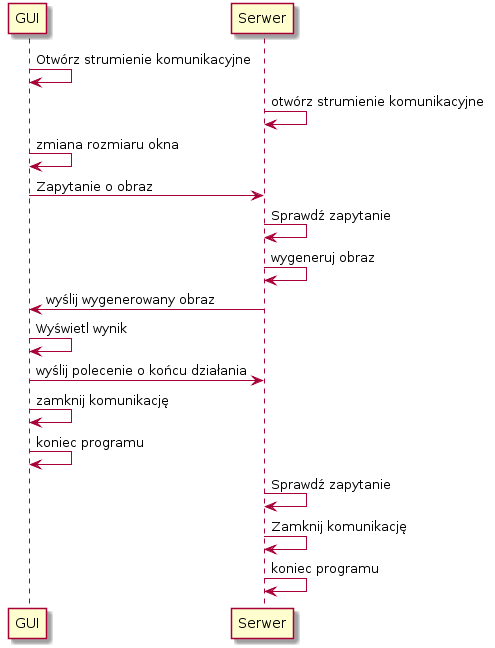
\includegraphics[width = 0.7\textwidth]{img/diagram.png}
\end{figure}
\subsection{Server}
Zasada podziału pracy w części serwerowej przedstawiona jest na poniższym diagramie.
Obraz dzielony jest na linie grubości 1 px. każdy wątek poza wątkiem głównym dostaję za zadanie obliczenie lini. Wątek główny ma za zadanie zebrać wszystkie wyliczone linie obrazu w odpowiedniej kolejności.
Kiedy obraz zostanie w pełni wygenerowany wątek główny który jest również odpowiedzialny za komunikację z GUI wysyła gotowy obraz do użytkownika.
Taka struktura podziału pracy sprawia że serwer musi działać przynajmniej na 2 wątkach, ponieważ wątek główny odpowiedzialny jest za komunikację oraz łączenie obrazu w całość, natomiast pozostałe wątki odpowiadają wyłącznie za generowanie danych.
\begin{figure}[H]
    \centering
    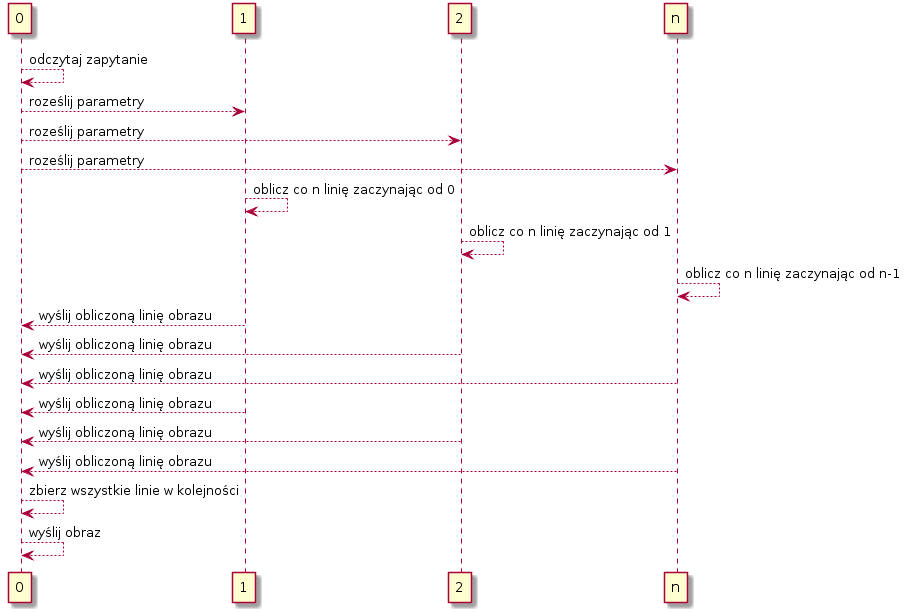
\includegraphics[width = \textwidth]{img/watki.png}
\end{figure}

Algorytm wyznaczania zbioru Mandelbrota opiera się na podnoszeniu do kwadratu liczby zespolonej i dodawaniu do niej stałej. Jeśli wartość tej liczby po podniesieniu do kwadratu jest mniejsza od 2, istnieje szansa, że punkt ten należy do zbioru. Aby to potwierdzić uzyskaną wartość ponownie podnosi się do kwadratu i dodaje tę samą stałą. Jeśli po odpowiednio dużej ilości iteracji wartość ta nie przekroczy 2, to punkt uznaje się za część zbioru, jeśli jednak wartość ta przekroczy 2, to dla danego punktu wybierany jest odpowiedni kolor w zależności od ilości iteracji przez które ten punkt miał wartość poniżej 2.

Prezentowany algorytm jest więc bardzo niezależny. teoretycznie nie ma przeszkód aby każdy piel liczony był niezależnie, jednak ze względu na prostotę implementacji, oraz łatwość rekonstrukcji obrazu, każdy wątek na raz liczy jedynie linię szerokości grubości 1 px i szerokości docelowego obrazu.

\subsection{GUI}
Interface użytkownika po połączeniu do serwera wysyła pierwsze zapytanie o wygenerowanie obrazu zbioru Mandelbrota.

Możliwa jest zmiana rozmiaru okna, oraz przybliżania części obrazu.
W trakcie zaznaczania lewym przyciskiem myszy obszaru do przybliżania zachowywane są proporcje ekranu.

Zaimplementowana została również funkcja cofania przybliżenia realizowana za pomocą prawego przycisku myszy.

Należy zwrócić uwagę, że dość łatwo jest zbliżyć się w takim stopniu do elementu obrazu że wartości szerokość okna na płaszczyźnie zespolonej nie może być dokładnie wyznaczona za pomocą liczby zmiennoprzecinkowej, a przy znacznym przybliżeniu obliczenia mogą zająć znacząco dłużej ze względu na konieczność zwiększania ilości iteracji dla każdego pixelu, aby zachować ostre krawędzie oraz odpowiednią paletę kolorów poza zbiorem.



\section{Przykłady działania aplikacji}
Po uruchomieniu aplikacji celem \textbf{run\_local} oczom użytkownika ukaże się
okno klienta oraz terminal wypełniony informacjami diagnostycznymi.\\

Przykładowa prezentacja:
\begin{figure}[H]
    \centering
    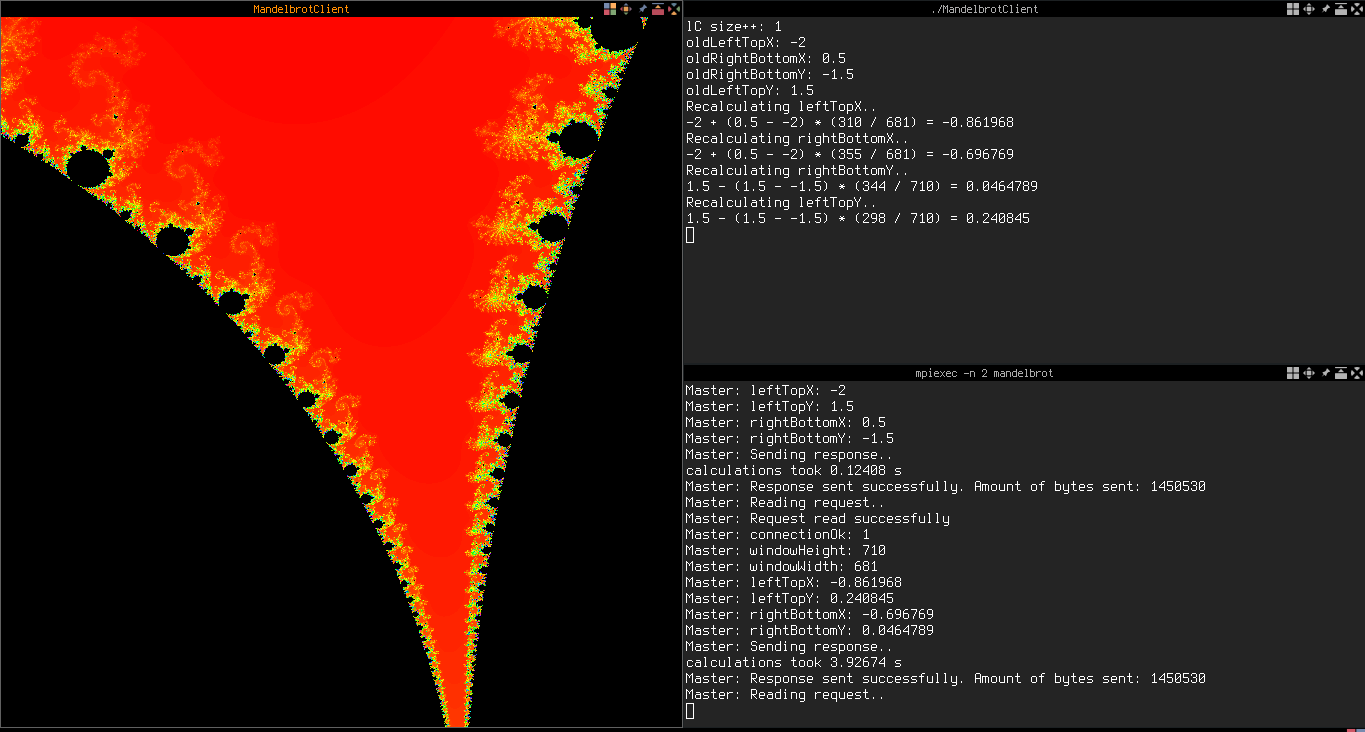
\includegraphics[width = \textwidth]{img/ex2.png}
\end{figure}

Jak można zaobserwować na poniższym obrazie aplikacja pozwala uzyskać znaczne przybliżenie na elementy zbioru.
\begin{figure}[H]
    \centering
    
\includegraphics[width = 0.7\textwidth]{img/ex3.png}
\end{figure}
\bibliography{references}
\bibliographystyle{plain}
\end{document}
